\documentclass[tikz,border=10pt]{standalone}
% No extra TikZ libraries needed.
\begin{document}
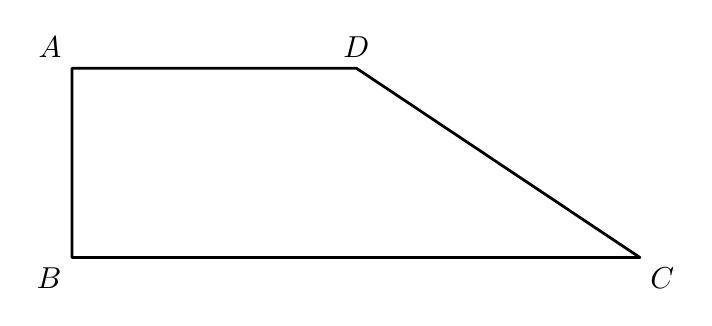
\begin{tikzpicture}[line join=round, line width=1.0pt, font=\fontsize{10.5}{12.6}\selectfont]
  % Vertices: scale s = 0.012719 cm/px, origin at B, y flipped
  \coordinate (A) at (0.000, 2.404);
  \coordinate (B) at (0.000, 0.000);
  \coordinate (C) at (7.212, 0.000);
  \coordinate (D) at (3.612, 2.404);

  % Quadrilateral ABCD, solid black, no fill
  \draw[black] (A) -- (B) -- (C) -- (D) -- cycle;

  % Labels
  \node[above left] at (A) {$A$};
  \node[above] at (D) {$D$};
  \node[below left] at (B) {$B$};
  \node[below right] at (C) {$C$};
\end{tikzpicture}
\end{document}